\begin{figure}[!b]
\centering
\begin{subfigure}{0.4\textwidth}
    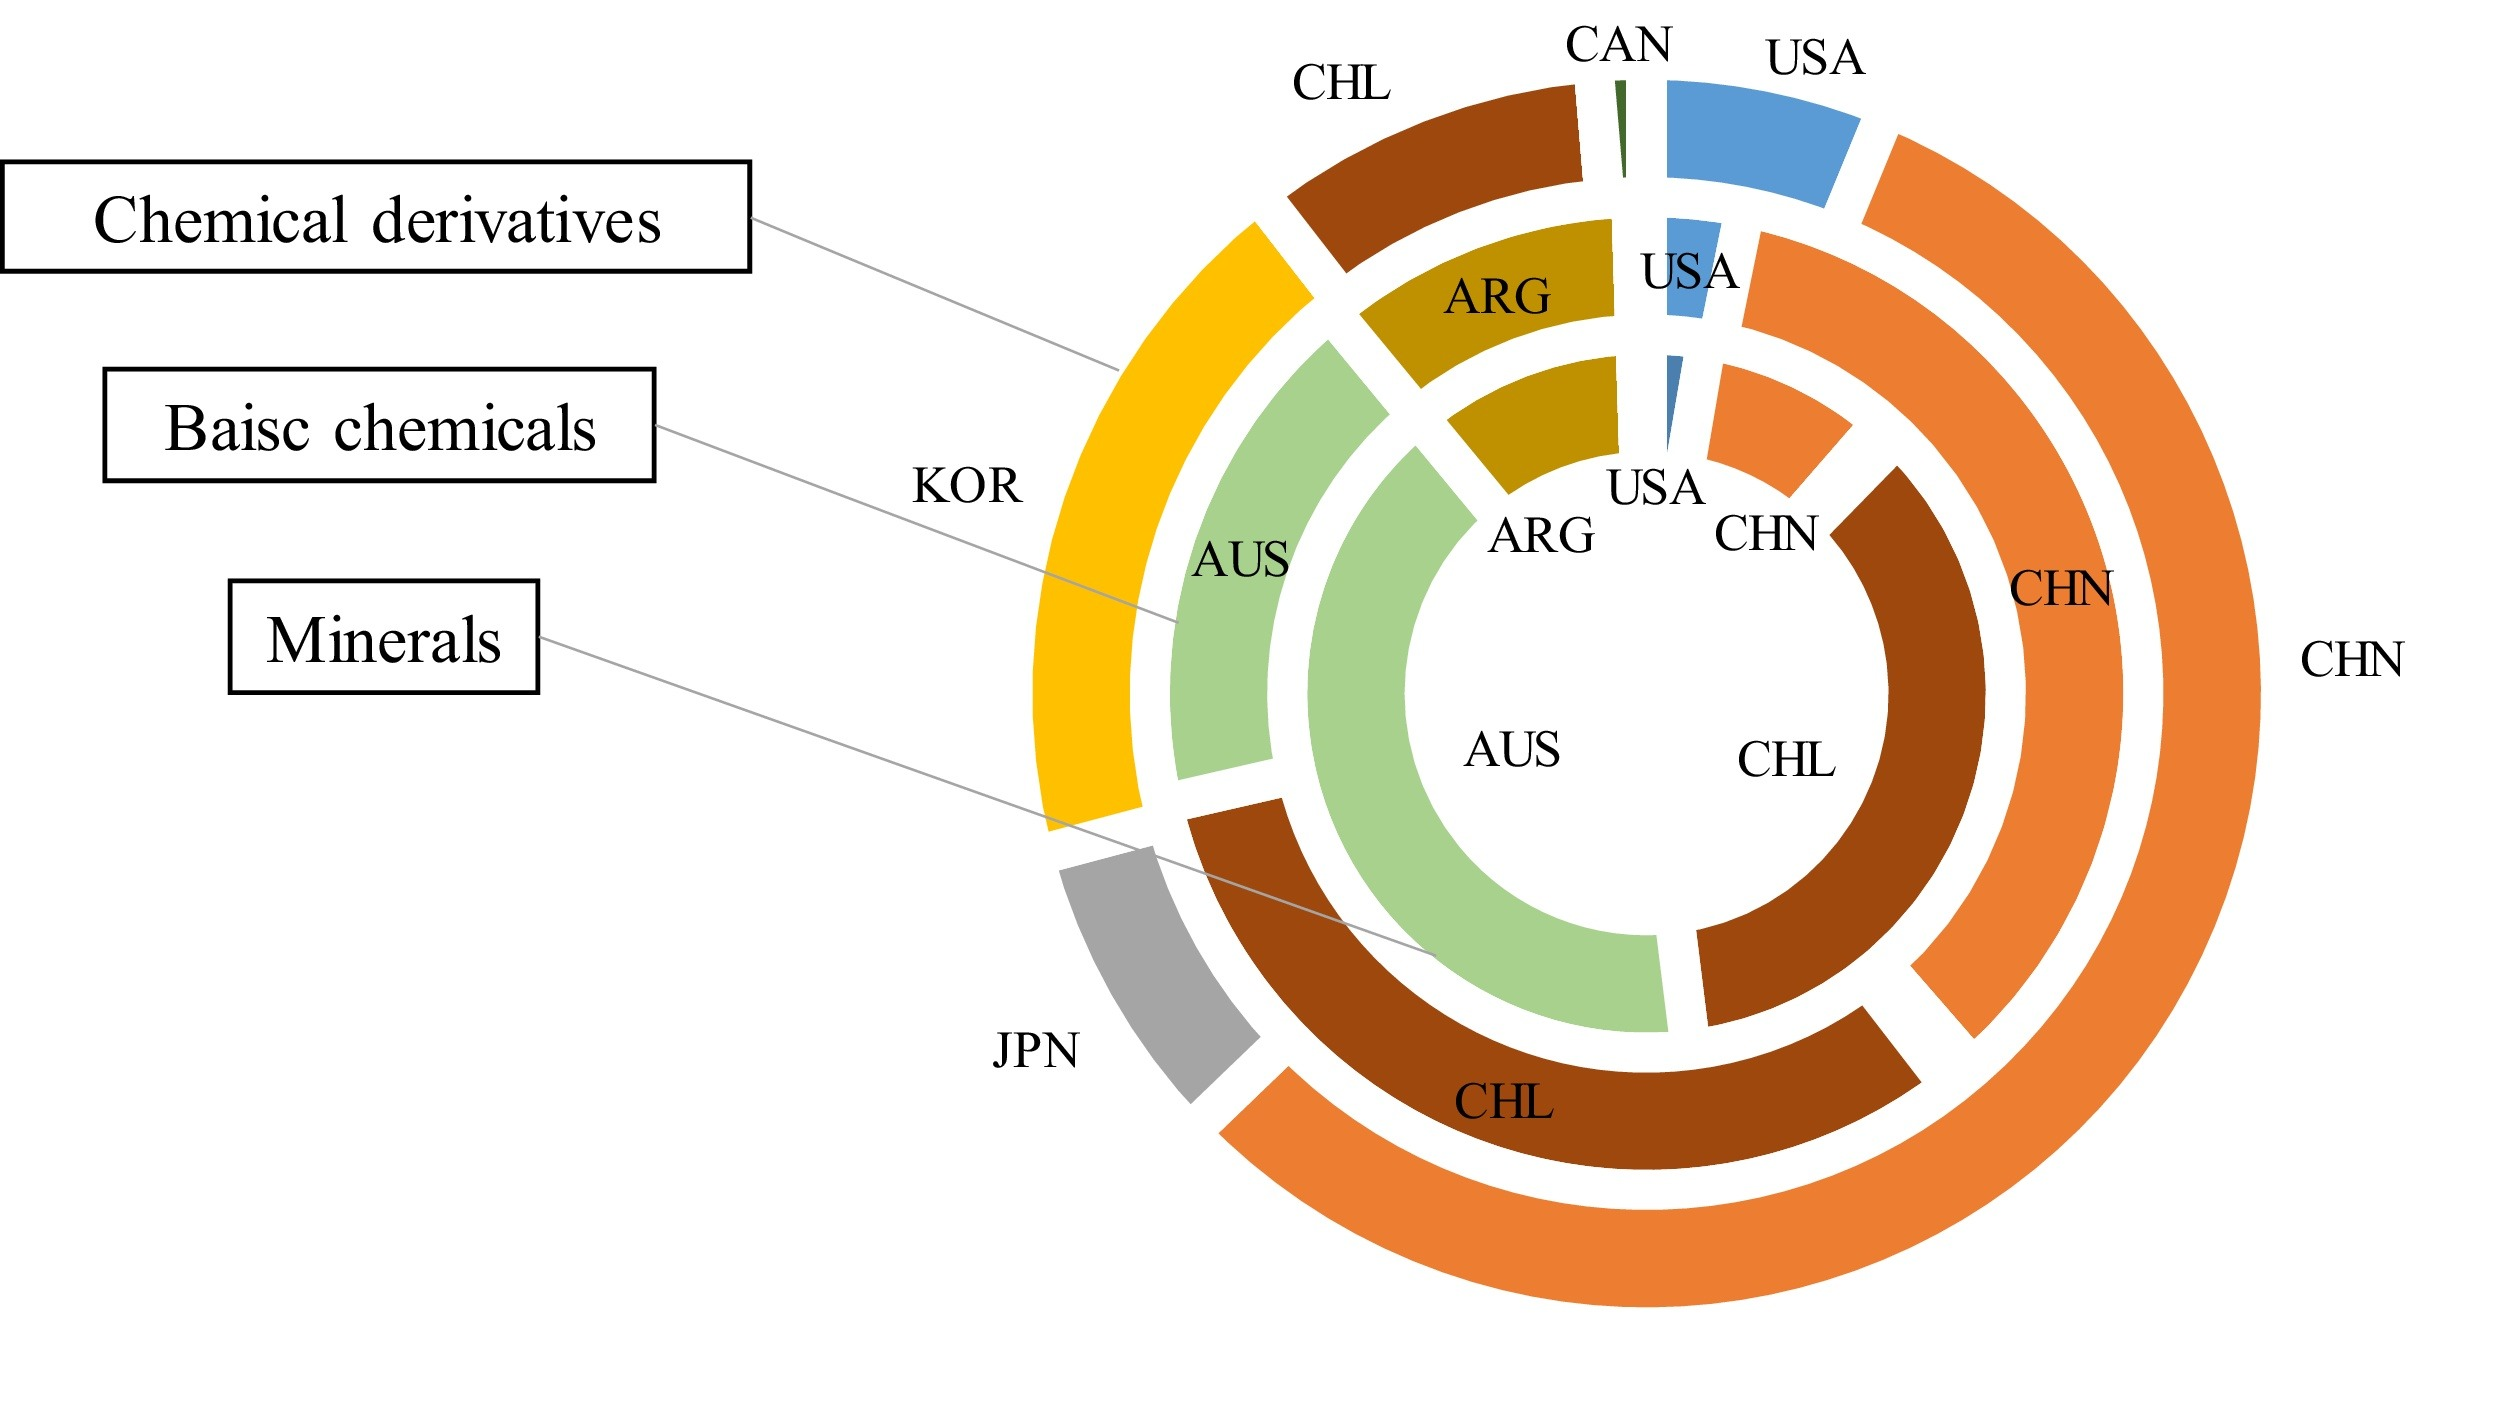
\includegraphics[width=\textwidth]{Images/supply_chain/1-s2.0-S0921344917301118-gr5_lrg.jpg}
    \caption{Répartition de l'extraction et du raffinage du lithium par pays}
    \label{fig:lithium_country}
\end{subfigure}
\hfill
\begin{subfigure}{0.4\textwidth}
    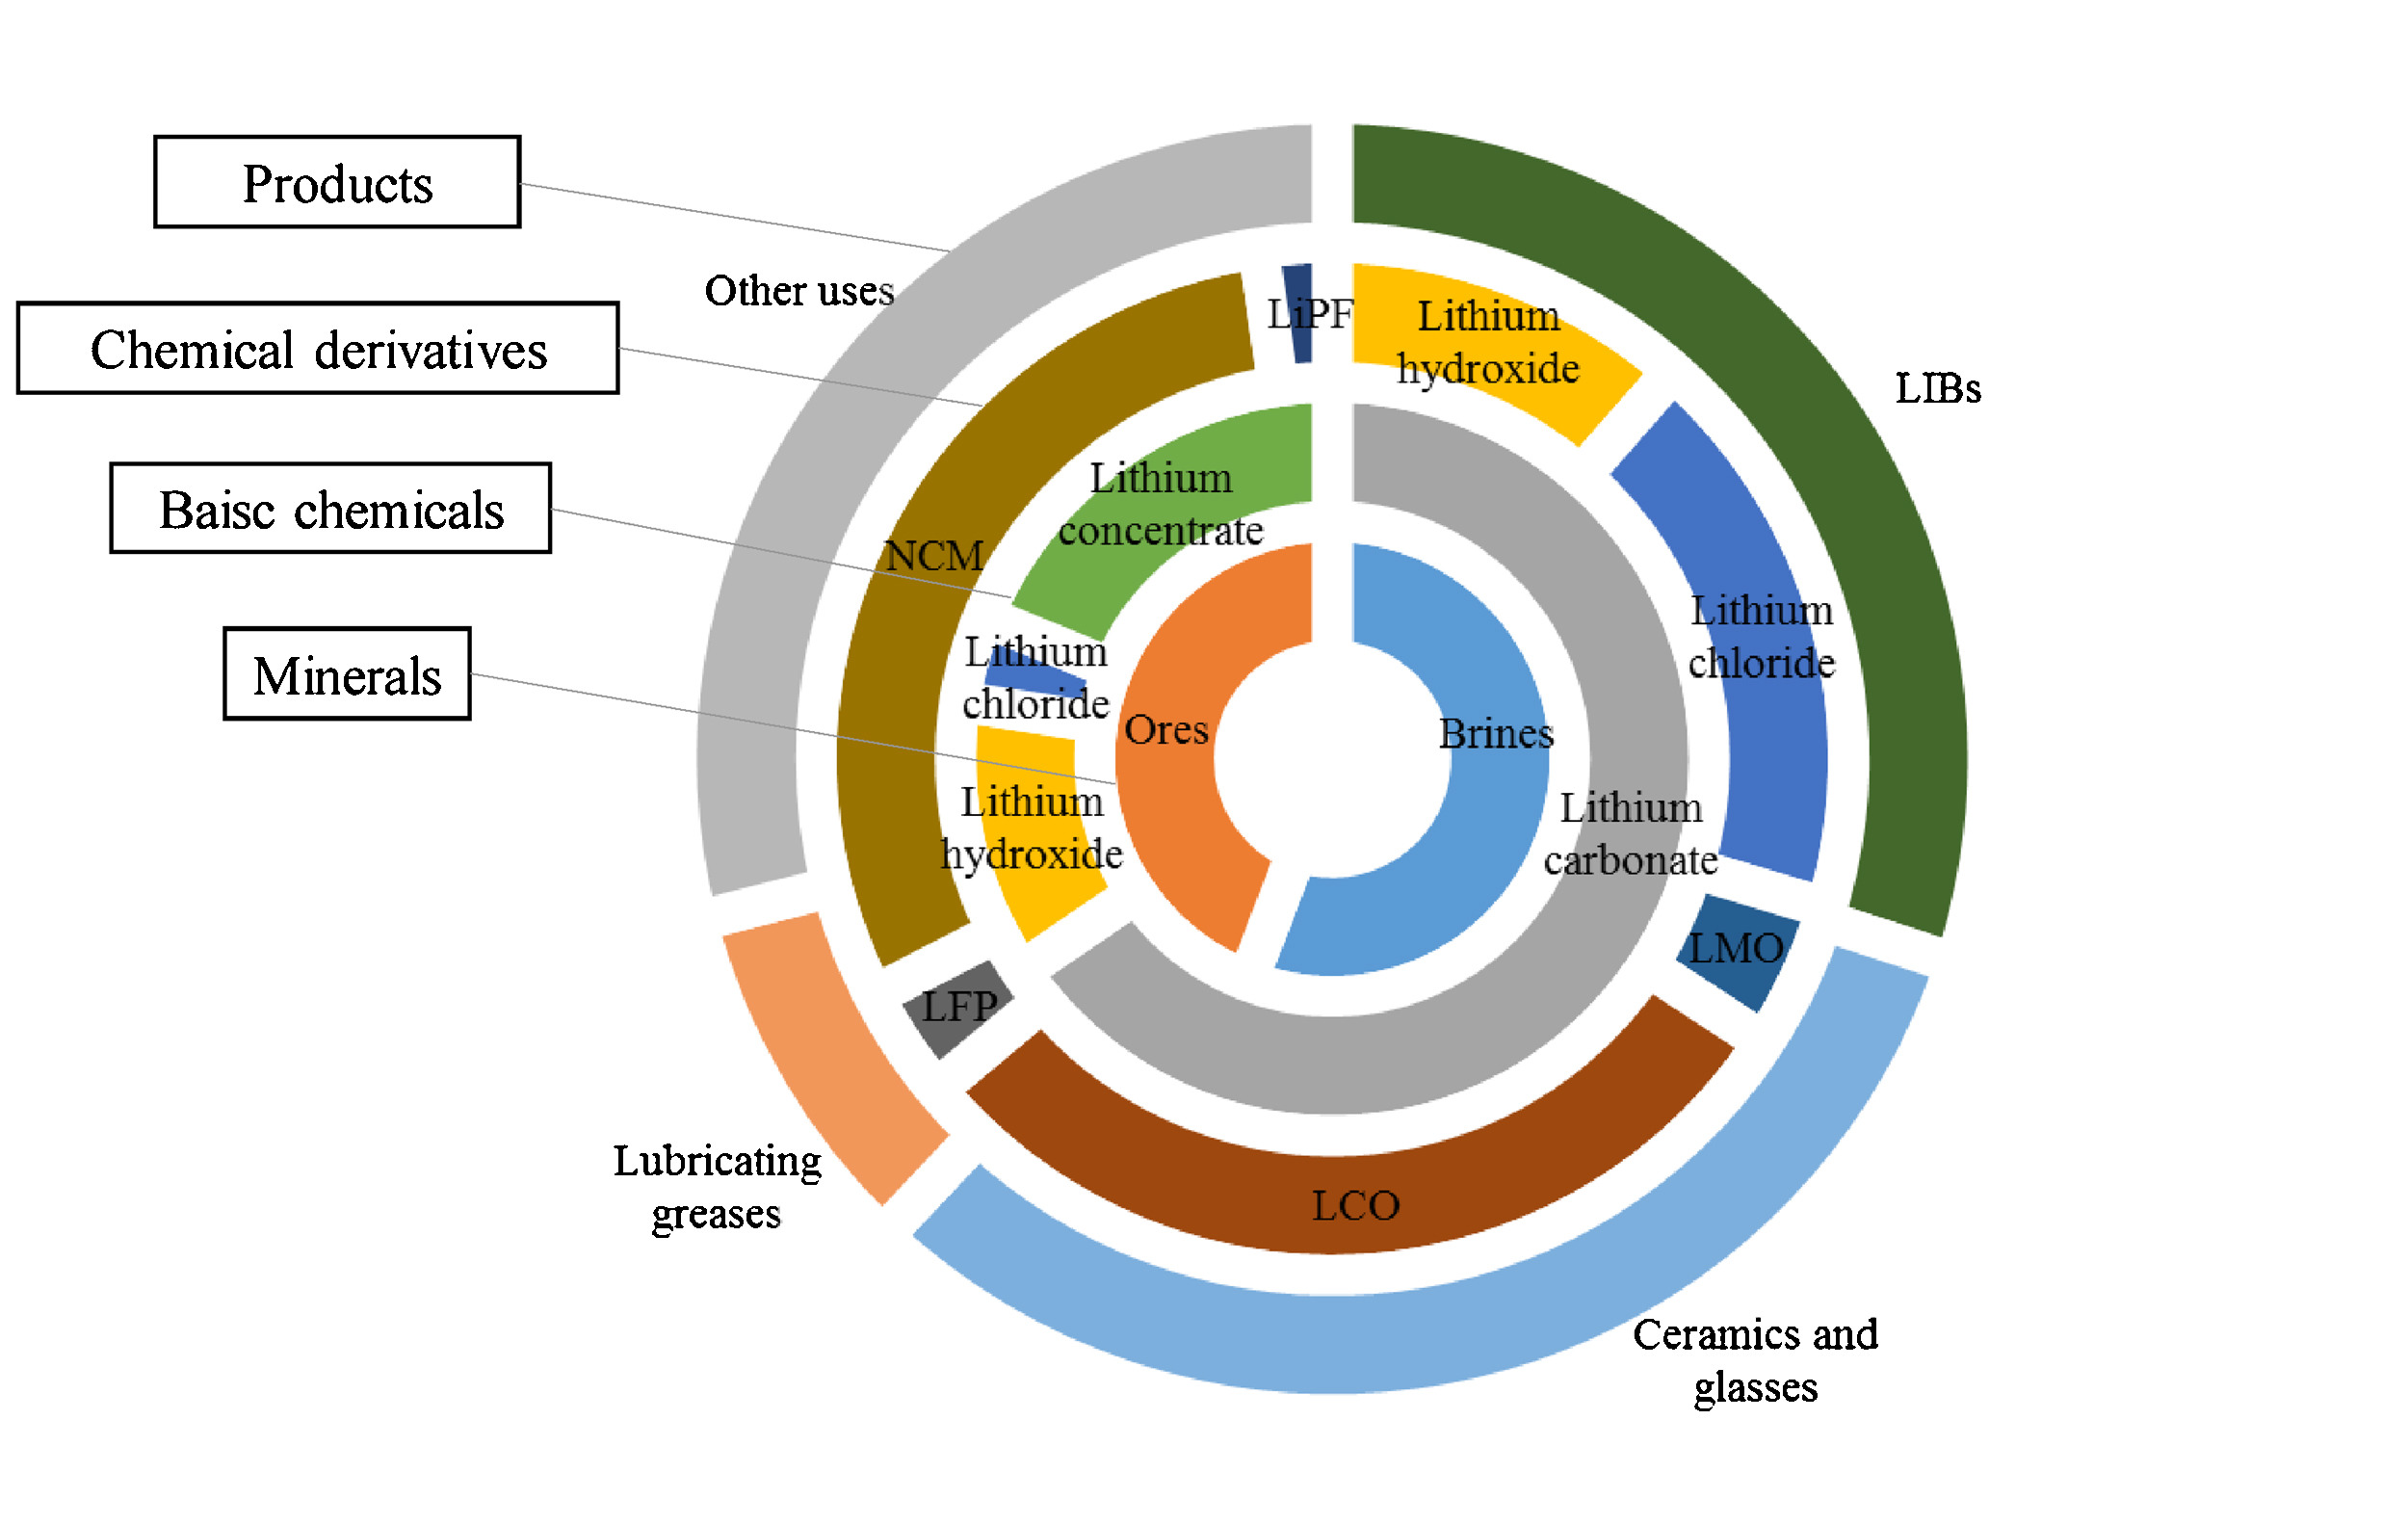
\includegraphics[width=\textwidth]{Images/supply_chain/1-s2.0-S0921344917301118-gr6_lrg.jpg}
    \caption{Répartition de la chaine de valeur du lithium par type de produits}
    \label{fig:lithium_type}
\end{subfigure}
\hfill
\begin{subfigure}{0.4\textwidth}
    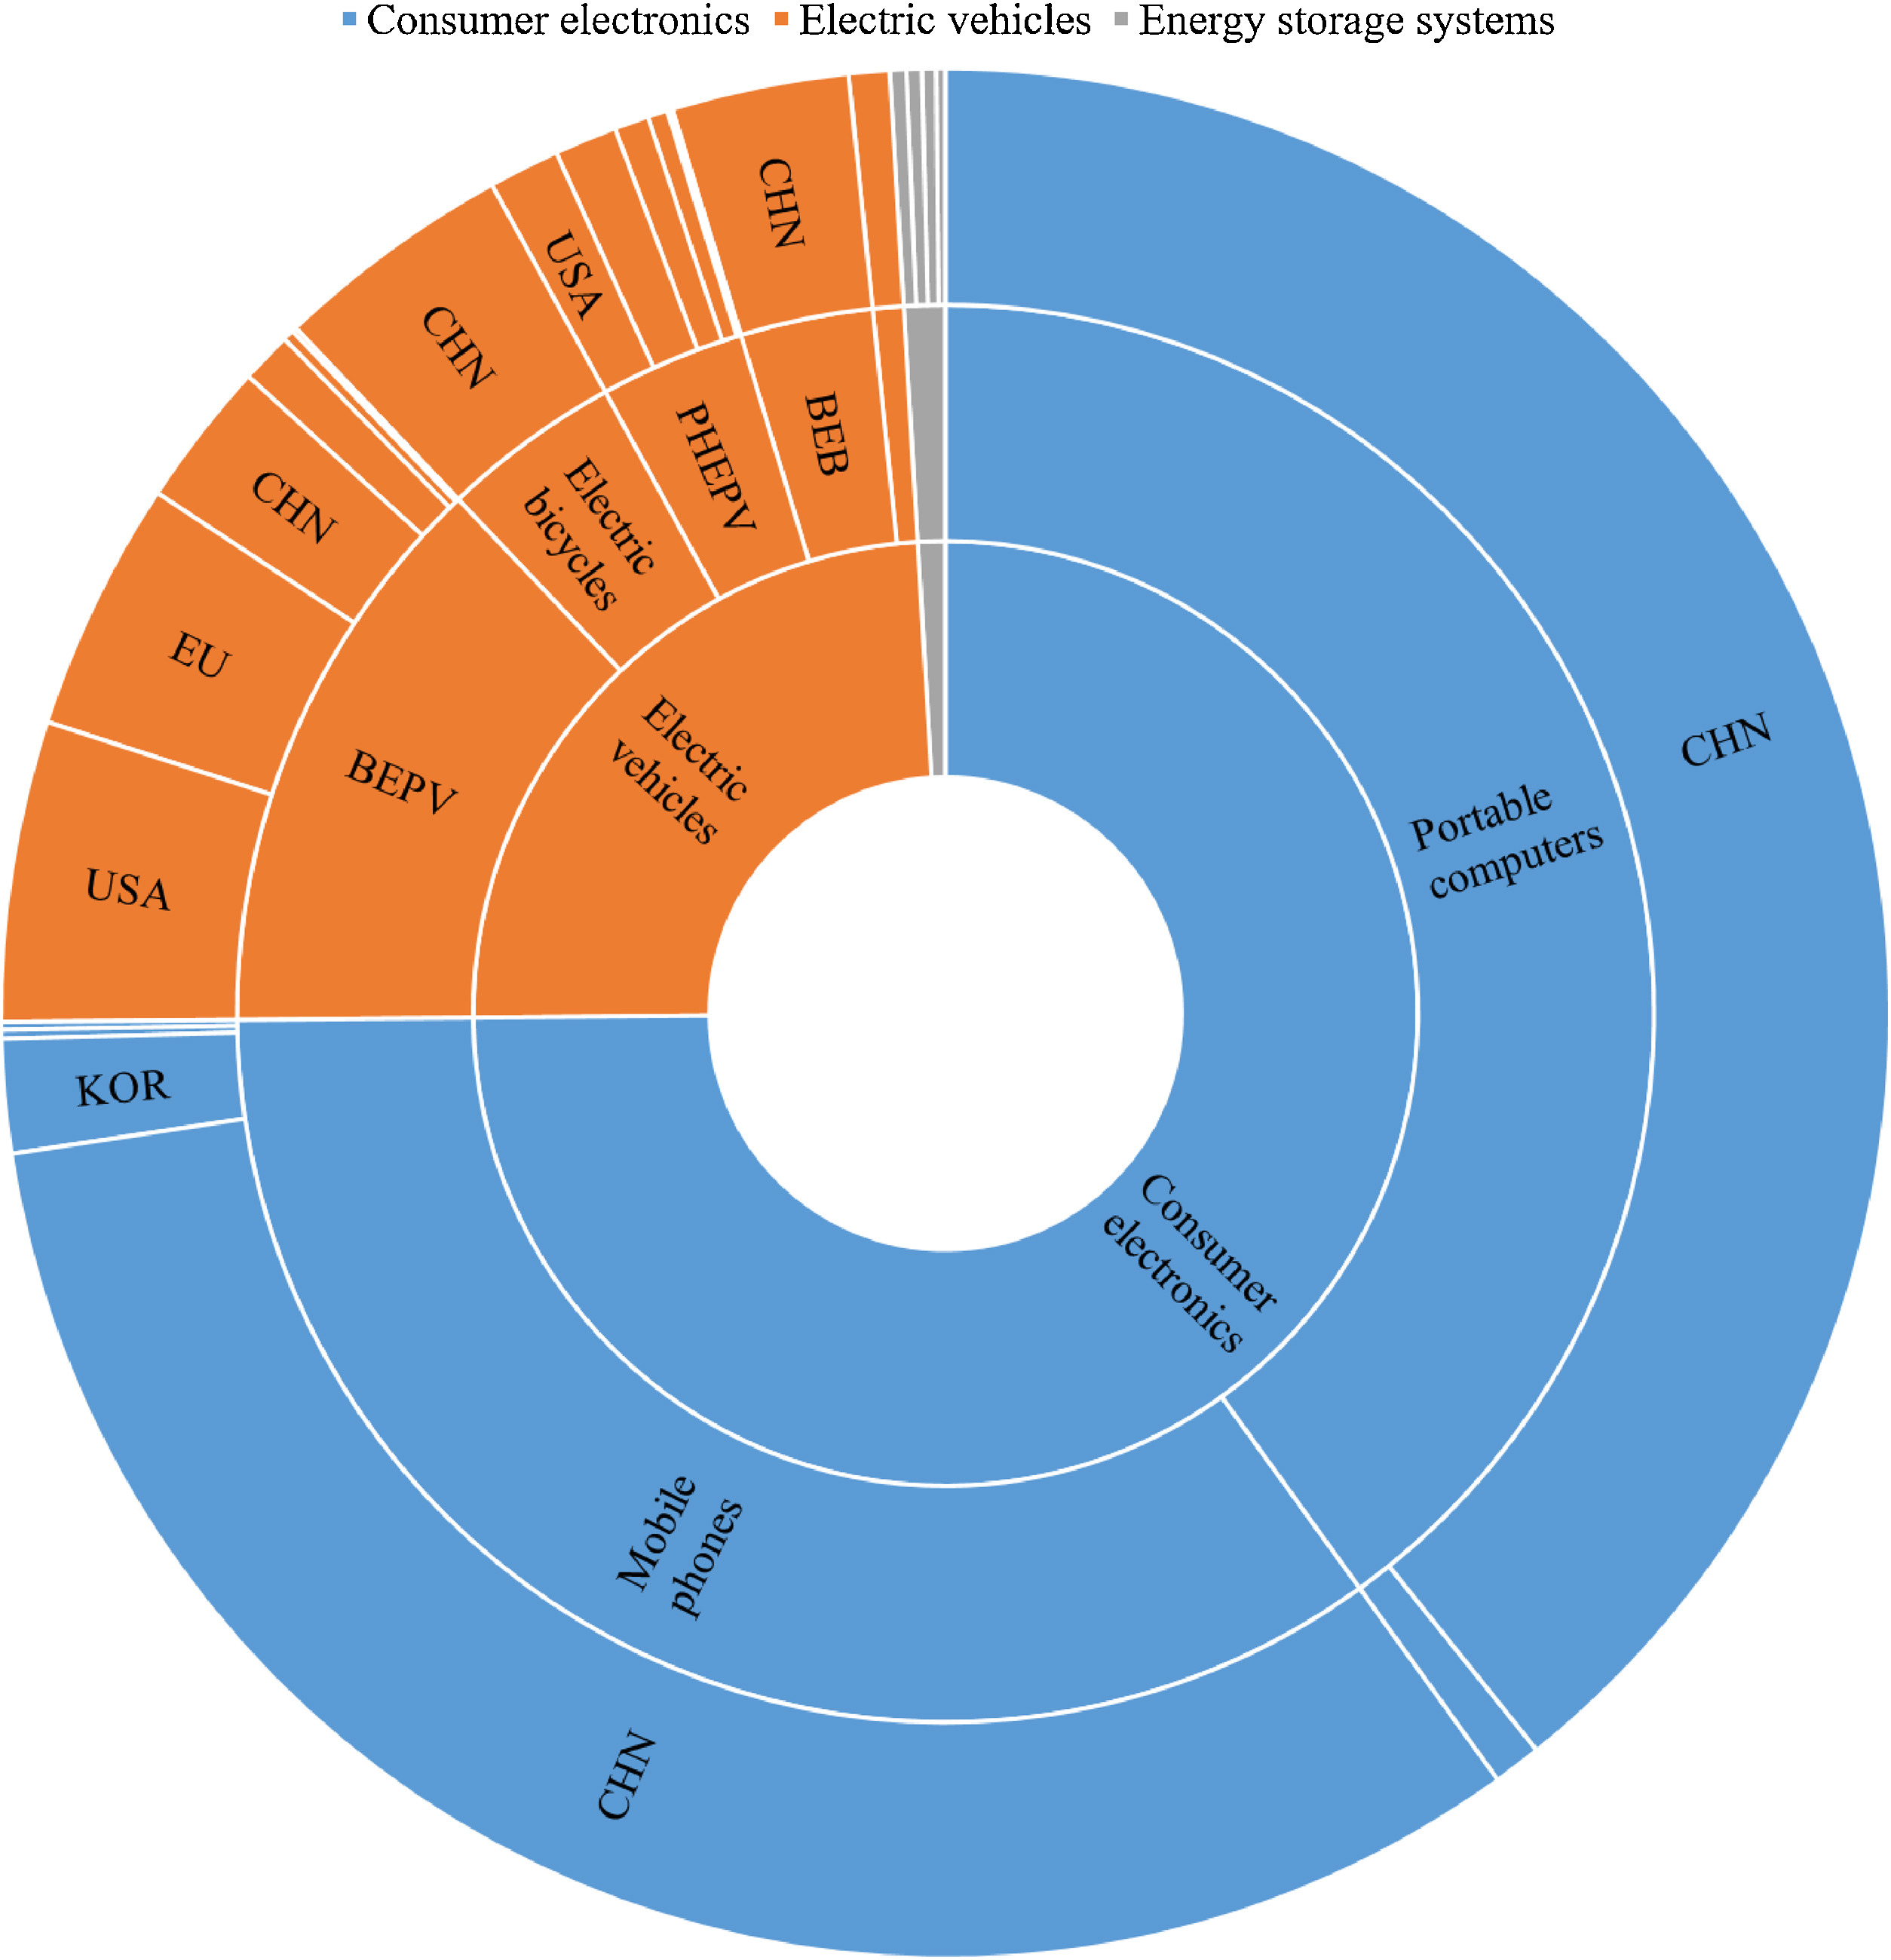
\includegraphics[width=\textwidth]{Images/supply_chain/1-s2.0-S0921344917301118-gr7_lrg.jpg}
    \caption{Répartition de la consommation de batterie lithium-ion (LIBs) par usage}
    \label{fig:LIB_use}
\end{subfigure}
        
\caption{Chaine d'approvisionnement issue du lithium (\cite{sun_tracing_2017})\\}
\caption*{Note : La chaine d'approvisionnement évolue très rapidement, les données présentées peuvent devenir obsolètes à moyen terme}
\label{fig:lithium_supply_chain}
\end{figure}

Les systèmes énergétiques décarbonés seront dépendants de chaînes d'approvisionnement plus complexes - illustré par la multiplicité des produits en figure \ref{fig:lithium_type}- avec une valeur ajoutée très importante à l'aval de l'extraction. Dans la continuité de la section précédente, cette section expose les enjeux géopolitiques autour de la maîtrise industrielle et technologique à l'aval de l'extraction.\smallbreak
Cette section présentera un état des lieux de l'industrie bas-carbone actuellement dominée par l'industrie chinoise. La figure \ref{fig:lithium_country} illustre l'importance de la Chine dans le raffinage du lithium, mais l'industrie chinoise a un poids bien plus important dans d'autres technologies bas-carbone.\smallbreak
Les enjeux géopolitiques dépendent de la capacité des industries à réagir à des évènements géopolitiques. Pour cette raison, cette section abordera les temporalités dans les chaînes d'approvisionnement. Les temps de déploiement de nouveaux site de production sur l'ensemble de la chaîne de valeur seront discutés : des temps très longs au niveau de l'extraction et relativement moyens pour les maillons de production proches de l'utilisation finale.\smallbreak
Enfin, cette section discutera de plusieurs leviers pour améliorer la sécurité et la résilience des approvisionnements. Elle abordera d'une part le rôle de la maîtrise technologique pour améliorer la substituabilité des métaux et d'autre part le rôle du recylage pour réduire les tensions d'approvisionnement.
